\documentclass{standalone}
\usepackage{tikz,pgf}

\begin{document}

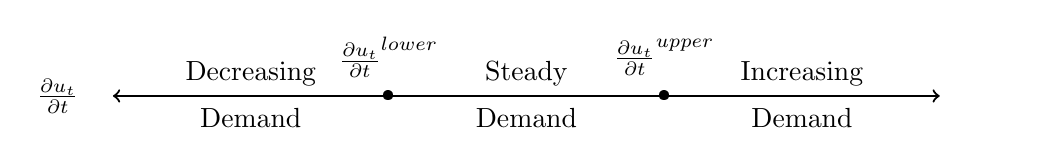
\begin{tikzpicture}[scale=7]

\node [draw=none] at (1,0.04) {Increasing};
\node [draw=none] at (1,-0.04) {Demand};

\node [draw=none] at (0.5,0.04) {Steady};
\node [draw=none] at (0.5,-0.04) {Demand};

\node [draw=none] at (0,0.04) {Decreasing};
\node [draw=none] at (0,-0.04) {Demand};

\node [draw=none] at (0.25,0.07) {$\frac{\partial u_t}{\partial t}^{\text{lower}}$};
\node [draw=none] at (0.75,0.07) {$\frac{\partial u_t}{\partial t}^{\text{upper}}$};

\foreach \Point in {0.25, 0.75}{
    \node[label={[label distance=1mm]:\rotatebox{0}{}}] at (\Point,0) {\textbullet};
}
\draw[thick,<->,color=black] (-0.25,0) -- (1.25,0); % Draw line
\node [draw=none] at (-0.35,0) {\bm{$\frac{\partial u_t}{\partial t}$}}; % Chart label
\node [draw=none] at (1.35,0)  {\color{white} $\frac{\partial u_t}{\partial t}$}; % Added to center chart

\end{tikzpicture}

\end{document}